\documentclass[a4paper]{article}
\usepackage[utf8]{inputenc}




\title{Pendolo reversibile - Caduta libera}
\author{Ali Matteo, Broggi Diana, Cantarini Giulia}
\date{ }

\usepackage{tabularx}
\usepackage{natbib}
\usepackage{graphicx}
%\usepackage[demo]{graphicx}
%\usepackage{subfig}
%\usepackage[margin=1.0in]{geometry}

\usepackage{tikz}
\usepackage{caption}
\usepackage{subcaption}
\usepackage{amsmath, amsthm}
\usepackage{hyperref}
\usepackage{mathrsfs}

\usepackage{pgfplots}
%\pgfplotsset{width=4cm,compat=1.9}

\theoremstyle{definition}
\newtheorem{rich}{richiamo matematico}[section]





%roba che crea comando per centrare immagine dentro immagine piu grande
%https://tex.stackexchange.com/a/308286
\newlength{\imagew}
\newlength{\imageh}
\newlength{\legendw}
\newlength{\legendh}
\newlength{\legendx}
\newlength{\legendy}
\newcommand{\graphicswithlegend}[6]{
	\setlength{\imagew}{#1}
	\settoheight{\imageh}{\includegraphics[width=\imagew]{#2}}
	
	\setlength{\legendw}{#3\imagew}
	\settoheight{\legendh}{\includegraphics[width=\legendw]{#4}}
	
	\setlength{\legendx}{\imagew}
	\addtolength{\legendx}{-\legendw}
	\addtolength{\legendx}{-#5\imagew}
	
	\setlength{\legendy}{\imageh}
	\addtolength{\legendy}{-\legendh}
	\addtolength{\legendy}{-#6\imageh}
	
	\includegraphics[width=\imagew]{#2}%
	\llap{
		\hspace{-\the\legendx}
		\raisebox{\legendy}{\includegraphics[width=\legendw]{#4}}
		\hspace{\the\legendx}
	}
}



\begin{document}
	\pagenumbering{arabic}
	\maketitle
	\section*{pendolo di Kater}
	Lo scopo di questa esperienza era quello di calcolare una stima dell'accelerazione di gravità mediante l'osservazione dei periodi di oscillazione del pendolo di Kater. Questo strumento presenta due masse in grado di scorrere lungo l'asta. Abbiamo usato come perno di rotazione entrambi i coltelli alternativamente per diverse configurazioni delle posizioni delle masse. Per misurare i periodi abbiamo impiegato una fotocellula collegata ad un cronometro che registrava il passaggio del pendolo.\\
	Si può dimostrare che, osservato un certo periodo T*, vale la relazione:
	\[T^{*} = 2\pi \sqrt{\frac{D}{g}}\] dove T* corrisponde ai periodi T1,periodo di una oscillazione rispetto al coltello 1, e T2, rispetto al coltello 2, in una configurazione (posizione delle masse relativa ai coltelli) del pendolo tale per cui essi si equivalgono. 
	\subsubsection*{procedura sperimentale e misurazioni}
	Per ricavare T* abbiamo eseguito le misure di T1 e T2 più volte per ogni posizione in cui la massa B veniva spostata, la massa A è rimasta fissa durante tutto l'esperimento. Nel corso di questa procedura i valori venivano inseriti in un programma in Python (il cui codice sorgente è consultabile al link in fondo alla pagina) per generare il grafico dei periodi medi T1 e T2 in funzione della distanza della massa B dal coltello 2
	\begin{figure}[!ht]
		\captionsetup{labelformat=empty}
		\makebox[1 \textwidth][c]{       %centering table
			\resizebox{0.56 \textwidth}{!}{   %resize table
				\includegraphics{relazione_Pendolo_Kater/computed_data/punti.png}
			} %close resize
		} %close centering
		\caption{\url{https://github.com/giiulia/relazione_pendolo_Kater}}
	\end{figure}

\noindent l'osservazione dello sviluppo di questo grafico ci ha aiutato ad individuare la direzione corretta per muovere la massa B al fine di ottenere delle misure vicine al punto di intersezione tra la curva del T1 e quella del T2.\\
Di seguito esponiamo le misure effettuate per ogni distanza di B dal coltello 2:\\\\
distanza 1 in metri:
\begin{table}[!ht]
	\centering
%	\input{relazione_Pendolo_Kater/computed_data/tableDistances1.tex}
\end{table}


\begin{figure}[!htbp]
	\makebox[1 \textwidth][c]{       %centering table
		\begin{tabular}{l|*{11}{c}}
			\hline
			\hline
			Periodo 1(s) & 1.9485 & 1.9483 & 1.9488 & 1.9489 & 1.9483 & 1.9484 & 1.9487 & 1.9487 & 1.9482 & \\
			\hline
			\hline
			Periodo 2(s) & 1.8306 & 1.83 & 1.8295 & 1.8286 & 1.8292 & 1.8298 & 1.8288 & 1.8287 & 1.829 & 1.8289\\
			\hline
			\hline
		\end{tabular}
		
	} %close centering
\end{figure}

\noindent distanza 2 in metri:
\begin{table}[!ht]
	\centering
%	\input{relazione_Pendolo_Kater/computed_data/tableDistances2.tex}
\end{table}

\begin{figure}[!htbp]
	\makebox[1 \textwidth][c]{ 
		\begin{tabular}{l|*{11}{c}}
			\hline
			\hline
			Periodo1 (s) & 1.9637 & 1.9638 & 1.9636 & 1.9636 & 1.9635 & 1.9633 & 1.9632 & 1.963 & 1.9634 & \\
			\hline
			Periodo2 (s) & 1.8614 & 1.8612 & 1.861 & 1.8612 & 1.8608 & 1.8606 & 1.8608 & 1.8611 & 1.8612 & 1.8612 & \\
			\hline
			\hline	
		\end{tabular}
	} %close centering
\end{figure}

\noindent distanza 3 in metri:
\begin{table}[!ht]
	\centering
%	\input{relazione_Pendolo_Kater/computed_data/tableDistances3.tex}
\end{table}


\begin{figure}[!htbp]
	\makebox[1 \textwidth][c]{ 
		\begin{tabular}{l|*{11}{c}}
			\hline
			\hline
			Periodo1 (s)& 1.9827 & 1.9824 & 1.9826 & 1.9822 & 1.9828 & 1.9825 & 1.9826 & 1.9828 & 1.9825 & \\
			\hline
			Periodo2 (s) & 1.9264 & 1.9274 & 1.9264 & 1.9263 & 1.927 & 1.9258 & 1.9258 & 1.9257 & 1.9271 & 1.927 & \\
			\hline
			\hline
		\end{tabular}
	} %close centering
\end{figure}

\noindent distanza 4 in metri:
\begin{table}[!ht]
	\centering
%	\input{relazione_Pendolo_Kater/computed_data/tableDistances4.tex}
\end{table}


\begin{figure}[!htbp]
	\makebox[1 \textwidth][c]{ 
        \begin{tabular}{l|*{11}{c}}
			\hline
			\hline
			Periodo1 (s)& 1.9884 & 1.9887 & 1.9879 & 1.9877 & 1.9877 & 1.9876 & 1.9876 & 1.9876 & 1.988 & \\
			\hline
			Periodo2 (s)& 1.9378 & 1.9381 & 1.9369 & 1.9379 & 1.9366 & 1.9386 & 1.9374 & 1.9357 & 1.9357 & 1.9367 & \\
			\hline
			\hline
		\end{tabular}
	} %close centering
\end{figure}

\noindent distanza 5 in metri:
\begin{table}[!ht]
	\centering
%	\input{relazione_Pendolo_Kater/computed_data/tableDistances5.tex}
\end{table}


\begin{figure}[!htbp]
	\makebox[1 \textwidth][c]{ 
		\begin{tabular}{l|*{11}{c}}
			\hline
			\hline
			Periodo1 (s) & 2.0279 & 2.0265 & 2.0271 & 2.0256 & 2.0244 & 2.0251 & 2.0241 & 2.0232 & 2.0226 & 2.0226 & \\
			\hline
			Periodo2 (s)& 2.0075 & 2.0074 & 2.0071 & 2.0061 & 2.0065 & 2.0063 & 2.0065 & 2.0061 & 2.0061 & \\
			\hline
			\hline
		\end{tabular}
	} %close centering
\end{figure}
.\\\\\\
\noindent distanza 6 in metri:
\begin{table}[!ht]
	\centering
	\input{relazione_Pendolo_Kater/computed_data/tableDistances6.tex}
\end{table}


\begin{figure}[!htbp]
	\makebox[1 \textwidth][c]{ 
		\begin{tabular}{l|*{11}{c}}
			\hline
			\hline
			Periodo1 (s)& 2.0227 & 2.0222 & 2.0221 & 2.0228 & 2.0221 & 2.0217 & 2.0218 & 2.0217 & 2.0217 & \\
			\hline
			Periodo2 (s)& 2.1072 & 2.1046 & 2.1035 & 2.1046 & 2.1032 & 2.1034 & 2.1043 & 2.1025 & 2.1039 & 2.1024 & \\
			\hline
			\hline
		\end{tabular}
		
	} %close centering
\end{figure}

	\begin{figure}[!htbp]
	\captionsetup{labelformat=empty}
	\caption{dist \(m_{A}\)= 0.159 metri}
	\makebox[1 \textwidth][c]{ 
		\begin{tabular}{c|cc}
			\hline
			\hline
			dist \(m_{B}\) (m) & Periodo 1 (s) & Periodo 2 (s)\\
			\hline
			1: \(0.2940 \pm 	0.0002 \)& \(	1.94853  \pm 0.00008\) &\(1.8293 \pm 0.0002\)\\
			2: \(0.2350 \pm  0.0002\)& \(1.96346 \pm  0.00009\) &\( 1.86105 \pm  0.00008\)\\
			3: \(0.1682 \pm  0.0001\)& \( 1.98257\pm  0.00006 \)& \( 	1.9265 \pm 0.0002\)\\
			4: \(0.1584 \pm  0.0002\) & \( 1.9879 \pm 0.0001\)& \( 1.9371 \pm 0.0003\)\\
			5: \(0.1024 \pm 0.0002 \)& \( 2.0066 \pm 0.0002 \)&\(	2.0249 \pm 0.0006\) \\
			6: \(0.0628 \pm  0.0003\)& \( 2.0221 \pm  0.0004 \) &\(2.1040 \pm 0.0004 \)\\
			\hline
			\hline
		\end{tabular}
		
	} %close centering
\end{figure}

	\subsubsection*{calcolo dell'accelerazione di gravità}
In seguito all'acquisizione di questi dati abbiamo selezionato le misure osservate per T1 e T2 più vicine (sia da destra che da sinistra) all'intersezione delle curve, la cui ordinata rappresenta il T* cercato. Le posizioni di B che ci hanno portati più vicino all'intersezione sono state la distanza 4 e la distanza 5.\\
Se inseriamo i valori medi dei periodi per queste due posizioni all'interno della fomula:
\[T^{*} = \frac{T_{2}(x_{4})T_{1}(x_{5})-T_{1}(x_{4})T_{2}(x_{5})}{T_{1}(x_{5})-T_{2}(x_{5})-T_{1}(x_{4})+T_{2}(x_{4})}\]

\makebox[\textwidth]{
	{
		\small
dove \(T_{1}(x_{4})=1.988s\), \(T_{2}(x_{4})=1.937s\), \(T_{1}(x_{5})=2.007s\), \(T_{2}(x_{5})=2.0249s\)
	}
}
.\\\\
otteniamo \(T*=2.0017 \pm 0.0002 s\). L'incertezza su T* è stata calcolata come 
\makebox[\textwidth]{
	{
		\small
\(\sigma_{T^{*}} = \sqrt{\left ( \frac{\partial T^{*}}{\partial T_{2}(x_{4})} \right )^{2}\sigma_{T2(x4)}^{2} + \left ( \frac{\partial T^{*}}{\partial T_{2}(x_{5})} \right )^{2} \sigma_{T2(x5)}^{2}+\left ( \frac{\partial T^{*}}{\partial T_{1}(x_{4})} \right )^{2} \sigma_{T1(x4)}^{2}+\left ( \frac{\partial T^{*}}{\partial T_{1}(x_{5})} \right )^{2} \sigma_{T1(x5)}^{2}}\)
 	}
}
.\\
\noindent Questo risultato ci permette di calcolare g con estrema precisione, difatti, se la distanza tra i due coltelli è D = 0.994m, l'accelerazione di gravità risulta:
\[g = \frac{4\pi ^{2}D}{(T^{*})^{2}} \qquad \sigma _{g} = \frac{8\pi ^{2}D}{(T^{*})^{3}}\sigma _{T}\]
\[g = 9.794 \pm 0.002 \frac{m}{s^{2}}\]
\subsubsection*{stima degli errori sistematici}
Abbiamo sottoposto questo primo risultato per g al test della compatibilità con il valore atteso di 9.81 \(\frac{m}{s^{2}}\), \(t= \frac{\left | g_{osservata} - g_{attesa} \right |}{\sigma_{g}} = 4\), un valore di t sopra al 2 indica che la stima da noi raggiunta è probabilmente affetta da errori sistematici.\\
Per quanto riguarda la formula utilizzata ad esempio, essa è una semplificazione del caso reale in quanto assume un angolo di oscillazione massimo infinitesimo e l'assenza dell'attrito dell'aria sul pendolo.\\
Abbiamo calcolato nuovamente g considerando un angolo di \(0.0861 \pm 0.0008 rad\) come \(\theta _{max}\). In questo caso la relazione tra T* e g è la seguente:

\[T^{*}_{1} = 2\pi \sqrt{\frac{D}{g}} \left (1+\frac{\theta ^{2}}{16} \right )\]
\makebox[\textwidth]{
	{
		\scriptsize
		con \(\theta\) in radianti
	}
}
usando questa formula \(g_{1} = \frac{4\pi ^{2}D}{T^{*2}}\left ( 1+\frac{\theta ^{2}}{16} \right )^{2} \pm \sqrt{\left ( \frac{\partial g}{\partial T} \right )^{2}\sigma _{T}^{2}+\left ( \frac{\partial g}{\partial \theta }\right )^{2}\sigma _{\theta }^{2} }=\)\\\(=9.803\pm0.002 m/s^{2}\). L'errore sistematico sulla prima misura di g era dunque pari a \( \left | g-g_{1} \right | =  0.009 m/s^{2}\), dello stesso ordine di grandezza di quello casuale.\\
L'incertezza riportata per \(g_{1}\) è dovuta solo ad errori casuali, per stimare l'errore sistematico legato all'ampiezza dell'angolo su questa nuova misura di g dobbiamo preseguire con lo sviluppo in serie di potenze, la formula per T* diventa:
\[ T^{*}_{2}= 2\pi \sqrt{\frac{D}{g}} \left (1+\frac{\theta ^{2}}{16}+\frac{9\theta ^{4}}{1024}+\frac{25\theta ^{6}}{16384} \right )\] 
dunque \( \left | g_{2}-g_{1} \right | =  9 \cdot 10^{-6} m/s^{2}\) è l'errore sistematico sulla stima di \(g_{1}\), trascurabile rispetto a quello casuale \( \rightarrow \quad g = g_{1} = 9.803 \pm 0.002 m/s^{2}\) è la nostra stima più accurata. Non prevediamo di aver commesso altri errori sistematici rilevanti, la nostra discussione si conclude qua.
\section*{caduta libera}
Un altro metodo per misurare g è osservare la caduta di un grave. L'esperimento prevedeva l'utilizzo di una struttura che lascia cadere una sferetta metallica e rileva il tempo di caduta tramite un sensore presente sul luogo di atterraggio.

\subsubsection*{procedura sperimentale e misurazioni}
A causa di un guasto del cronometro dell'apparato siamo stati costretti a rilevare l'intervallo di tempo attraverso un procedimento aletrnativo. Abbiamo fissato una fotocellula e, sotto di essa, allineato una seconda fotocellula libera di scorrere lungo un'asta verticale per poter regolare la distanza fra i due gates.\\

\noindent Riportiamo le misure effettuate per le diverse altezze di partenza in metri, misurate come distanza fra le fotocellule, e i relativi tempi di caduta in secondi:\\\\\\\\\\

\noindent altezza 1:

\begin{table}[!htbp]
	\centering
	\input{relazione_caduta_libera/tabelle/tableHeights1.tex}
\end{table}

\begin{table}[!htbp]
	\centering
	\input{relazione_caduta_libera/tabelle/tableTimes1.tex}
\end{table}

\noindent altezza 2:

\begin{table}[!htbp]
	\centering
	\input{relazione_caduta_libera/tabelle/tableHeights2.tex}
\end{table}

\begin{table}[!htbp]
	\centering
	\input{relazione_caduta_libera/tabelle/tableTimes2.tex}
\end{table}
\noindent altezza 3:

\begin{table}[!htbp]
	\centering
	\input{relazione_caduta_libera/tabelle/tableHeights3.tex}
\end{table}
\begin{table}[!htbp]
	\centering
	\input{relazione_caduta_libera/tabelle/tableTimes3.tex}
\end{table}
\noindent altezza 4:

\begin{table}[!htbp]
	\centering
	\input{relazione_caduta_libera/tabelle/tableHeights4.tex}
\end{table}
\begin{table}[!htbp]
	\centering
	\input{relazione_caduta_libera/tabelle/tableTimes4.tex}
\end{table}
\noindent altezza 5:	

\begin{table}[!htbp]
	\centering
	\input{relazione_caduta_libera/tabelle/tableHeights5.tex}
\end{table}
\begin{table}[!htbp]
	\centering
	\input{relazione_caduta_libera/tabelle/tableTimes5.tex}
\end{table}
.\\\\\\\\\\\\\\\\\\\\
\noindent altezza 6:	

\begin{table}[!htbp]
	\centering
	\input{relazione_caduta_libera/tabelle/tableHeights6.tex}
\end{table}

\begin{table}[!htbp]
	\centering
	\input{relazione_caduta_libera/tabelle/tableTimes6.tex}
\end{table}


\begin{figure}[!htbp]
	\captionsetup{labelformat=empty}
	\caption{Tabella1}
	\makebox[1 \textwidth][c]{ 
		\begin{tabular}{c|c}
			\hline
			\hline
			altezza (m) & tempo di caduta (s)\\
			\hline
			1: \(0.603 \pm 0.0003\) &\(0.315 \pm 0.002\)\\
			2:  \(0.584 \pm  0.0003\)& \(0.309 \pm  0.002\)\\
			3:  \(0.557 \pm 0.0004\)& \( 0.295 \pm  0.003\)\\
			4: \(0.505 \pm  0.0003\)& \( 0.287 \pm  0.002\)\\
			5:\( 0.451 \pm 0.0003\)&  \(0.270 \pm 0.002\)\\
			6: \(0.396 \pm  0.0005\) &\(0.248 \pm   0.002\)\\
			\hline
			\hline
		\end{tabular}
	} %close centering
\end{figure}

\begin{figure}[!ht]
	\makebox[1 \textwidth][c]{       %centering table
		\resizebox{0.90 \textwidth}{!}{   %resize table
			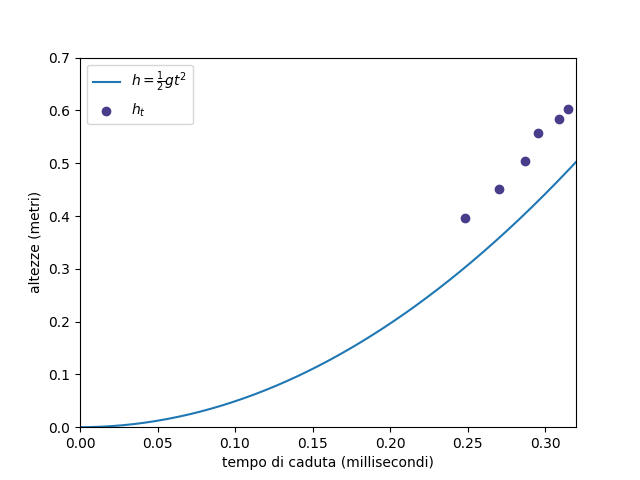
\includegraphics{relazione_caduta_libera/computed_data/parabola.png}
		} %close resize
	} %close centering
	
\end{figure}

\noindent La funzione \(h = \frac{1}{2}g t^{2}\) in azzurro ricavata con \(v_{0} = 0\) esprime una relazione lineare tra l'altezza di partenza ed il quadrato del tempo di caduta; perciò abbiamo eseguito l'interpolazione dei dati in Tabella 2.a al fine di stimare il valore del coefficiente \(\frac{2}{g}\)\\

\begin{figure}[!htbp]
	\captionsetup{labelformat=empty}
	\caption{Tabella2.a}
	\makebox[1 \textwidth][c]{ 
		\begin{tabular}{c|c}
			\hline
			\hline
			x: altezza (m) & y: tempo di caduta\(^{2}\) (\(s^{2}\))\\
			\hline
			1: \(0.603 \pm 0.0003\) &\(0.099\pm 0.001\)\\
			2:  \(0.584 \pm  0.0003\)& \(0.096 \pm 0.001\)\\
			3:  \(0.557 \pm 0.0004\)& \(  0.087 \pm 0.002 \)\\
			4: \(0.505 \pm  0.0003\)& \(  0.083 \pm  0.001 \)\\
			5: \( 0.451 \pm 0.0003\)&  \( 0.073 \pm  0.001\)\\
			6: \(0.396 \pm  0.0005\) &\(0.062 \pm  0.001\)\\
			\hline
			\hline
		\end{tabular}
	} %close centering
	\caption{\(\sigma_{t^{2}} = 2t\sigma_{t}\)}
\end{figure}
.\\\\
stime dei parametri della retta ricavati dall'interpolazione con il metodo dei minimi quadrati pesati:
\[B = \frac{\sum w_{i}\sum w_{i}x_{i}y_{i}-\sum w_{i}x_{i}\sum w_{i}y_{i}}{\Delta } \pm \sqrt{\frac{\sum w_{i}}{\Delta }} =0.177 \pm 0.006 s^{2}/m\]
\[A = \frac{\sum w_{i}x_{i}^{2}\sum w_{i}y_{i}-\sum w_{i}x_{i}\sum w_{i}x_{i}y_{i}}{\Delta } \pm \sqrt{\frac{w_{i}x_{i}^{2}}{\Delta }} = -0.008 \pm 0.003 s^{2}\]

\makebox[\textwidth]{
	{
		\normalsize
		\(\Delta = \sum (w_{i}y_{i}^{2})\sum w_{i}-(\sum w_{i}y_{i})^{2}\)\\
\( w_{i} = \frac{1}{\sigma_{ti}^{2}}\) poichè \(\sigma_{ti} >> \sigma_{hi}\)
}
}\\

\begin{figure}[!ht]
	\captionsetup{labelformat=empty}
	\makebox[1 \textwidth][c]{       %centering table
		\resizebox{0.90 \textwidth}{!}{   %resize table
			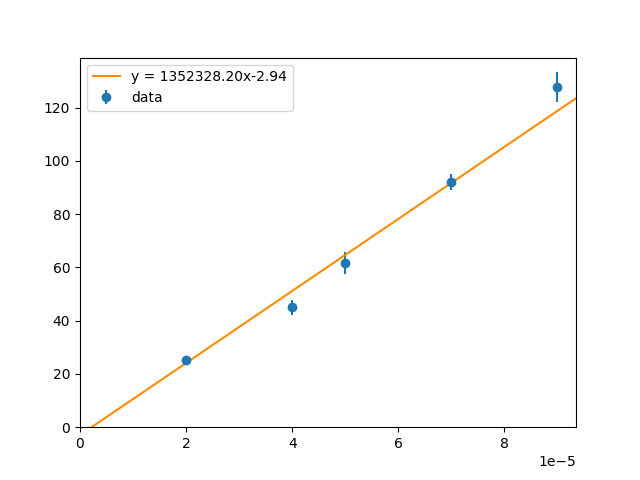
\includegraphics{relazione_caduta_libera/computed_data/retta.png}
		} %close resize
	} %close centering
\end{figure}

\noindent Infine, abbiamo calcolato l'accelerazione di gravità attraverso la formula che descrive il moto per \(v_{0} = 0\) \[g = \frac{2}{B} \pm \frac{2}{B^{2}}\sigma_{B} = 11.3 \pm 0.4 \frac{m}{s^{2}}\]

\subsubsection*{stima degli errori sistematici}
La stima di g ottenuta non è particolamente accurata, come ci aspettavamo dal grafico di \(h_{(t)}\):
\[t= \frac{\left | g_{osservata} - g_{attesa} \right |}{\sigma_{g}} = 3.7\]
 L'errore commesso pare di tipo sistematico, abbiamo supposto che fosse l'ipotesi di \(v_{0} = 0\). La tecnica di misurazione eseguita, a differenza dello strumento che avremmo dovuto utilizzare inizialmente, non permetteva di rilevare l'istante in cui la pallina cominciava a cadere: la partenza veniva effettuata leggermente al di sopra della prima fotocellula. Supponiamo un sollevamento \(\Delta{h}\) pari a \(1 \pm 0.1\)cm, durante il quale la pallina ha acquistato una \(v = \sqrt{2g\Delta{h}} = 0.44 \pm 0.02\frac{m}{s}\) prima di raggiungere la prima fotocellula.\\\\\\\\
Queste considerazioni ci hanno portato a tracciare un grafico atteso (sempre in azzurro) differente dal precedente:






\begin{figure}[!ht]
	\captionsetup{labelformat=empty}
	\makebox[1 \textwidth][c]{       %centering table
		\resizebox{0.90 \textwidth}{!}{   %resize table
			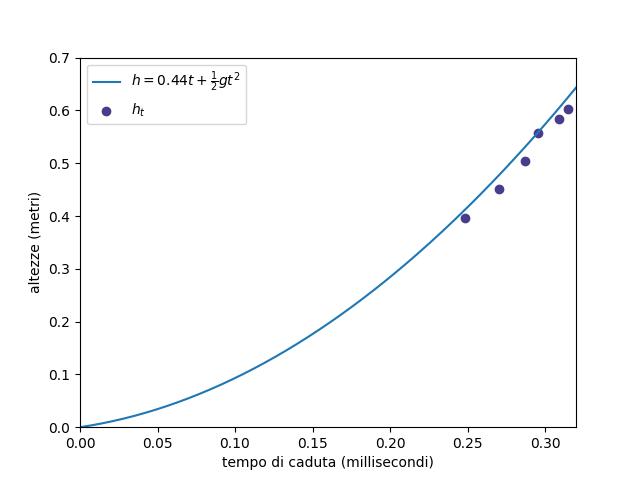
\includegraphics{relazione_caduta_libera/computed_data/parabola_corretta.png}
		} %close resize
	} %close centering
	\caption{la funzione che descrive il fenomeno è stata corretta per \(v_{0}\neq 0\)}
\end{figure}

\noindent notiamo che i dati si accordano molto meglio con la parabola che rappresenta \(h = 0.44t + \frac{1}{2}gt^{2}\).\\
Nella tabella seguente correggiamo i valori di h di un fattore \(-v_{0}t\) e le relative incertezze propagando anche l'errore sistematico sulla stima di \(v_{0}\).

\begin{figure}[!htbp]
	\captionsetup{labelformat=empty}
	\caption{Tabella2.b}
	\makebox[1 \textwidth][c]{ 
		\begin{tabular}{c|c}
			\hline
			\hline
			y: altezza-\(v_{0}\)t (m) & x: tempo di caduta\(^{2}\) (\(s^{2}\))\\
			\hline
			1: \(0.4639 \pm0.007\) &\(0.099\pm 0.001\)\\
			2:  \(0.4474 \pm   0.007\)& \(0.096 \pm 0.001\)\\
			3:  \( 0.4270 \pm 0.007\)& \(  0.087 \pm 0.002 \)\\
			4: \(0.3781 \pm  0.006\)& \(  0.083 \pm  0.001 \)\\
			5: \(0.3317 \pm0.006 \)&  \( 0.073 \pm  0.001\)\\
			6: \(  0.2865 \pm 0.005\) &\(0.062 \pm  0.001\)\\
			\hline
			\hline
		\end{tabular}
	} %close centering
	\caption{con \(v_{0} = 0.44 \pm 0.02 \frac{m}{s}\)}
\end{figure}
\noindent Notiamo che con questa correzione, che porta con se un errore sistematico poichè non conosciamo con certezza quale era la velocità inizale della pallina, \(\sigma_{hi} >> \sigma_{ti}\) dunque questa volta consideriamo trascurabile l'incertezza sui tempi al quadrato.\\\\
\noindent L'interpolazione dei dati che considerano una velocità iniziale diversa da 0 porta ai seguenti risultati (le formule adoperate sono le stesse, abbiamo usato i dati della Tabella2.b):
\[B_{corretto}=4.9 \pm 0.2 m/s^{s} \qquad A=-0.02  \pm 0.02 m\]

\begin{figure}[!ht]
	\captionsetup{labelformat=empty}
	\makebox[1 \textwidth][c]{       %centering table
		\resizebox{0.90 \textwidth}{!}{   %resize table
			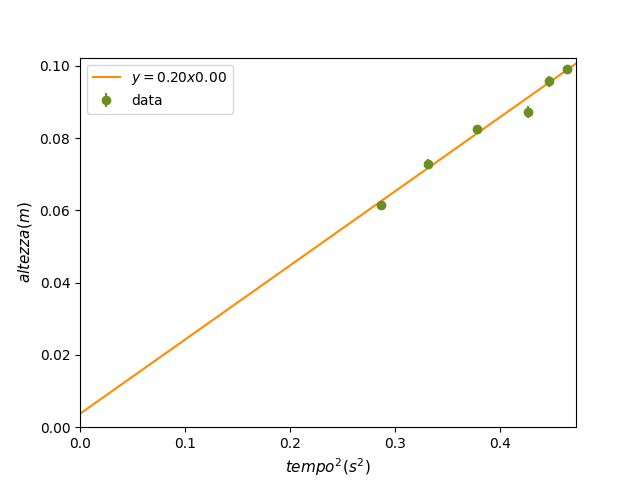
\includegraphics{relazione_caduta_libera/computed_data/retta_corretta.png}
		} %close resize
	} %close centering
\end{figure}

\noindent Procediamo dunque calcolando g con \(B_{corretto}\): \( g= 2B \pm 2\sigma_{B} = 9.8 \pm 0.4 m/s^{2}\). L'errore sistematico commesso sulla prima stima per g è stimabile con:\\ \(\left | g_{corretta} - g\right |=1.5 m/s^{2}\), decisamente non trascurabile.\\ 
\noindent Non prevediamo di aver commesso ulteriori errori sistematici importanti, la nostra stima per l'accelerazione di gravità è dunque \( g=9.8 \pm 0.4 m/s^{2}\).\\\\

	\makebox[\textwidth]{
	{	
		\small
		L'elaborazione dei dati è stata eseguita tramite un programma in Python
	}
}
	\makebox[\textwidth]{
	{	
		\small
 il cui codice è consultabile al seguente link:
	}
}
	\makebox[\textwidth]{
	{	
		\small
\url{https://github.com/giiulia/relazione_caduta_libera}
	}
}



\end{document}